% !TeX spellcheck = en_GB
\documentclass[main.tex]{subfiles}

\begin{document}
\chapter{Methods}
\lhead{Methods}
\label{chap:methods}

\section{Benchmarking named entity recognition}
\subsection{Evaluation of NER}
\label{subsec:nereval}
As explained in Section \ref{subsec:annoschemes}, all datasets used in the project supply an annotation label in IOB format \cite{ramshaw1995IOB} for each word in each sequence.
Comparing a sequence of true annotations and predictions, there are a number of potential error patterns as both the span and the type of the entity is to be guessed, see Table~\ref{tab:eval}.
\begin{table}[H]
    \footnotesize
    \centering
    \begin{tabular}{l|llllll}
        Sentence                    & Gaul & is & divided & into & three & parts.\\
        True annoation              & B-LOC & O & O & O & O & O \\\hline
        I (TP): Complete match      & B-LOC & O & O & O & O & O \\
        II (FP): Spurious entity    & B-LOC & O & O & O & O & B-MISC \\
        III (FN): Missing entity    & O     & O & O & O & O & O \\
        IV: Wrong type              & B-ORG & O & O & O & O & O \\
        V: Wrong boundary           & B-LOC & I-LOC & O & O & O & O \\
        VI: Wrong type and boundary & B-ORG & I-ORG & O & O & O & O
    \end{tabular}
    \caption{
        The different outcomes of a prediction when related to the ground truth.
        This categorization and naming is taken from \cite{batista2018eval}.
        The first three simple cases can be translated to true positives, false positives and false negatives, when considering only one entity type at a time.
    }
    \label{tab:eval}
\end{table}\noindent
In our evaluation, the simple and strict approach of the CoNLL-2003 shared task evaluation was followed, explained as:

''Precision is the percentage of named entities found by the learning system that are correct.
Recall is the percentage of named entities present in the corpus that are found by the system.
A named entity is correct only if it is an exact match of the corresponding entity in the data file.''
\cite[Sec 2.4]{tjang2003conll}

Using the terminology of Table~\ref{tab:eval}, these measures are, assuming the predictions and ground truth both contain at least one positive label, defined for each class (e.g. LOC) as
\begin{equation}
    \label{eq:precrec}
    \text{Precision} = \frac{\text{\# case I}}{\text{\# case I} + \text{\# case II}},\quad \text{Recall} = \frac{\text{\# case I}}{\text{\# case I} + \text{\# case III}}.
\end{equation}
From these class level metrics, global values of precision and recall were reported using the \emph{micro average}, that is, by aggregating the number of prediction outcomes (I, II, III) across classes before using formulae \eqref{eq:precrec}.
In the report, every reference to an average of metrics over NER classes refers to this micro average.
Thus, using this approach, the error types IV, V and VI are discriminated\footnotemark.
\footnotetext{
    Using this approach, the cases IV and VI in Table~\ref{tab:eval} would for the evaluation of the LOC class be treated as case III and for the evaluation of the ORG class be treated as case II.
    V would, similarly, be counted as both a case II and III for ORG.
    Such errors would thus be judged harshly in the global metrics and not show up in any way as partial corrects for any of the classes.
}

Following previous literature, the main score on which the system performance was judged is the F1 score, the harmonic mean of precision of recall;
\begin{equation}
    \label{eq:f1}
    \text{F1} = \dfrac{2}{\text{Precision}^{-1} + \text{Recall}^{-1}}
\end{equation}
The reported scores were obtained using a Python sequence evaluation library \cite{seqeval}, also used by the original LUKE paper and DaNLP, with whom comparisons are made.

Two of the three used datasets contains MISC annotation,s and existing literature disagrees on whether to consider this class in evaluations with DaNLP arguing
''We are only reporting the scores on the LOC, ORG and PER entities as the MISC category has limited practical use'' \cite[Sec. ''Benchmarks'' in NER page]{danlp2021}.
We trained all models with the MISC annotation and also include it in our evaluations.
When comparing with models trained without MISC, a non-MISC average F1 score is also reported (by treating all MISC predictions as null class predictions).
\subsection{Fine-tuning English LUKE}
Yamada et al. benchmark LUKE on named entity recognition using the CoNLL-2003 dataset \cite{yamada2020luke}.

Reproduction of these results were attempted by obtaining the pretrained LUKE models from Yamada et al.'s software repository.
The same hyperparameters as Yamada et al. were used and are shown along with and technical details in Table~\ref{tab:params}.

The fine-tuning procedure was repeated five times for each of the two released LUKE models, called \emph{large} and \emph{base}, to examine variability in the downstream training.
%%% Horrible footnote manipulation - it works, dont touch it! %%%
\addtocounter{footnote}{1}
\footnotetext{\label{foot:fnt}
    The pre-trained models were downloaded on 17/02-2021 from the LUKE software repository:
    \url{https://github.com/studio-ousia/luke/tree/6feefe657d97d2f847ace87f61f23b705f75d2aa\#released-models} 
} 
\begin{table}[H]
    \centering
    \begin{tabular}{l|rr}
        Pre-trained model
                                    & LUKE large\textsuperscript{\ref{foot:fnt}}\
                                                & LUKE base\textsuperscript{\ref{foot:fnt}}\\\hline
        Pre-trained model parameters & $483\ctp 6$ & $253\ctp 6$\\
        Pre-trained model entity vocabulary & $500\ctp3$ & $500\ctp3$\\
        Learning rate               & $10^{-5}$ & $5\ctp{-5}$\\
        Effective batch size        & 16 & 16\\
        Numeric precision           & \multicolumn{2}{l}{Mixed FP16/FP32 (Nvidia APEX)}\\
        Training code               & \multicolumn{2}{l}{PyTorch-based \code{luke}-repository\protect\footnotemark}\\
        Software version            & \multicolumn{2}{l}{Python 3.6, PyTorch 1.2}
    \end{tabular}
    \caption{Hyperparameters used to fine-tune LUKE large and LUKE base on the CoNLL-2003 dataset.}
    \label{tab:params}
\end{table}

\footnotetext{
    The repository \url{github.com/studio-ousia/luke} was cloned at commit-SHA \code{6feefe6}, installed and used for the fine-tuning.
}
\subsection{Off-the-shelf, Danish models}
\label{sec:exidan}
A number of Danish NER models that are publily available and usable by NLP practitioners were collected and evaluated on the testing datasets of the three Danish NER annotations considered in Section \ref{subsec:daNERdata}:
DaNE, Plank and WikiANN.

Most of the models were found through DaNLP \cite{danlp2021} and a number of them are introduced in Section \ref{sec:nlpda}.

\setlist{itemsep=.5em}
\begin{itemize}
    \item \textbf{DaNLP da-BERT}: The da-BERT model \cite{botxo2019dabert} fine-tuned for NER on DaNE by DaNLP.
    \item \textbf{NERDA m-BERT}: The multilingual BERT base released by the original Google Research BERT team \cite{devlin2019bert} fine-tuned by NERDA \cite{kjeldgaard2020nerda} on DaNE.
    \item \textbf{NERDA Ælæctra}: The transformer Ælæctra, released by Malte Højmark-Bertelsen, \cite{bertelsen2020lctra} fine-tuned by NERDA on DaNE.
    \item \textbf{DaCy}: An adaption of version 3 of the SpaCy framework \cite{honnibal2020spacy} to Danish by Kenneth Enevoldsen including fine-tuning of on DaNE \cite{enevoldsen2020dacy}.
        Both the medium and large versions are benchmarked, using the base and large multilingual RoBERTa \cite{conneau2020unsupervised} models, respectively.
        This 2021 model, large version, is the currently reported state of the art.
    \item \textbf{DaNLP spaCy}: SpaCy, version 2, adapted to Danish by DaNLP and fine-tuned on DaNE.
    \item \textbf{DaNLP Flair}: The Flair framework \cite{akbik2019flair} also adapted to Danish by DaNLP and fine-tuned on DaNE.
    \item \textbf{Polyglot}: A NLP framework supporting a wide range of tasks in many languages including NER in 40 different languages.
        The NER model is fine-tuned using automatic, language-agnostic annotations generated from Wikipedia and Freebase link structures \cite{rfou2015polyglot}.
    \item \textbf{daner (DKIE Stanford CRF)}: An application of the Stanford CoreNLP Conditional Random Field (CRF) NER classifier \cite{manning2014corenlp} released by Leon Derczynski asa part of the DKIE project \cite{derc2014dkie}.
    The model was trained on NER annotations produced at ITU on the Danish Dependency Treebank (DDT) corpus \cite{kromann2003ddt}.
    The released Java-based NER tool is called \code{daner}\footnotemark.
\footnotetext{
    The repository is at \url{github.com/ITUnlp/daner}
}
\end{itemize}
\setlist{noitemsep}
\noindent
The weights of all these finished NER models were downloaded and evaluated in accordance with Section \ref{subsec:nereval}.
The code for performing inference for all the models on the three datasets and measuring the F1 scores can be found in the module \code{reproduction.danish\_ner} in the DaLUKE repository\footnotemark.
The reproduction was performed using Python version 3.7.10 and the dependency versions defined in the requirements of DaNLP and NERDA.
\footnotetext{
    The reproduction code is available here:
    \url{github.com/peleiden/daluke/tree/master/reproduction/danish_ner}.
}
\section{DaLUKE}

\subsection{Pretraining Methodology and Hyperparameters}%
\label{sub:dalpre}
Our pretraining approach followed the one used by Yamada et al, as described in Section \ref{subsec:lukepre}, with four key differences:
\begin{enumerate}
    \item The entity-augmented Danish Wikipedia described in section \ref{subsec:entaug} was used.
    \item
        Entity-aware self-attention was used in the pretraining, as this was expected to positively impact the modeling of knowledge.
        This speculation is tested in Section~\ref{subsec:selfatt}.
    \item 
        The model followed the architecture of BERT base instead of BERT large, and weights were initialized from BotXO's da-BERT \cite{botxo2019dabert} as no Danish RoBERTa or BERT large is available.
        An ablation study on this transfer learning from da-BERT is introduced in Section~\ref{subsec:dabertexp}.
        Because of this, token embeddings and contextualized representations both reside in a 768 dimensional latent space rather than the 1024 dimensions used by LUKE.
        DaLUKE also has 12 attention blocks rather than 24.
        \cite[Sec. 3.4]{yamada2020luke}
    \item
        The entity vocabulary, consisting of all mentioned Wikipedia articles, was limited in the English LUKE for computational efficiency \cite[Sec. 3.4]{yamada2020luke}.
        We do not perform such limiting as the number of mentioned Wikipedia articles is much smaller in the Danish corpus.
        An experiment of limiting the vocabulary is explained in Section~\ref{subsec:entvocexp}.
\end{enumerate}
Due to the memory intensive nature of the transformer architecture, we followed Yamada et al. and used gradient accumulation over multiple subbatches within each batch, that is, each parameter update consists of multiple forward passes of the model.

As with LUKE, the cross entropy loss is calculated using equation \ref{eq:crossentropyloss} for each classification task, with the only difference being that the final loss is the average rather than the sum of the individual task losses.
This effectively just scales the loss and has no effect on the learning if the learning rate is adjusted accordingly.

The hyperparameters used for pretraining are shown in Table \ref{tab:pretrain-hyper}.
These were chosen based on informal experiments, as structured hyperparameter search was not within time frame.
\begin{table}[H]
    \centering
    \begin{tabular}{l|r}
        Parameter  &    Value\\\hline
        Epochs     & 150\\
        Batch size &    4080\\
        Peak learning rate & $3\ctp{-4}$\\
        LR warmup steps prop. & $ 6\pro $\\
        Mask prob. for words & $ 15\pro $\\
        Mask prob. for entities & $ 15\pro $\\
        Dropout & $ 0.1 $\\
        Weight decay & $ 0.01 $\\
        AdamW $ \beta_1 $ & $ 0.9 $\\
        AdamW $ \beta_2 $ & $ 0.999 $\\
        AdamW $ \epsilon $ & $ 10^{-6} $
    \end{tabular}
    \caption{Hyperparameters used for DaLUKE pretraining.}\label{tab:pretrain-hyper}
\end{table}\noindent
LUKE follows BERT and increases its learning rate linearly from 0 to the peak learning rate followed by a linear decrease to 0 for the rest of the learning rate - the slanted triangle learning rate (STLR). \cite{devlin2019bert, yamada2020luke, howardruder2018universal}

For pretraining, DaLUKE also employs linear warmup for the first 6\pro\ of parameter updates, after which it decreases polynomially with a power of $ \sqrt{3} $ and a final learning rate of one tenth the peak learning rate.
This results in a more aggressive decrease in learning rate after the warmup period but a slightly higher learning rate in the final steps compared to STLR.
This was used as the amount of available compute was not known in advance, and this approach would work well with both early stopping and continued training.
The learning rate development is shown on Figure \ref{fig:lr}.
\begin{figure}
    \centering
    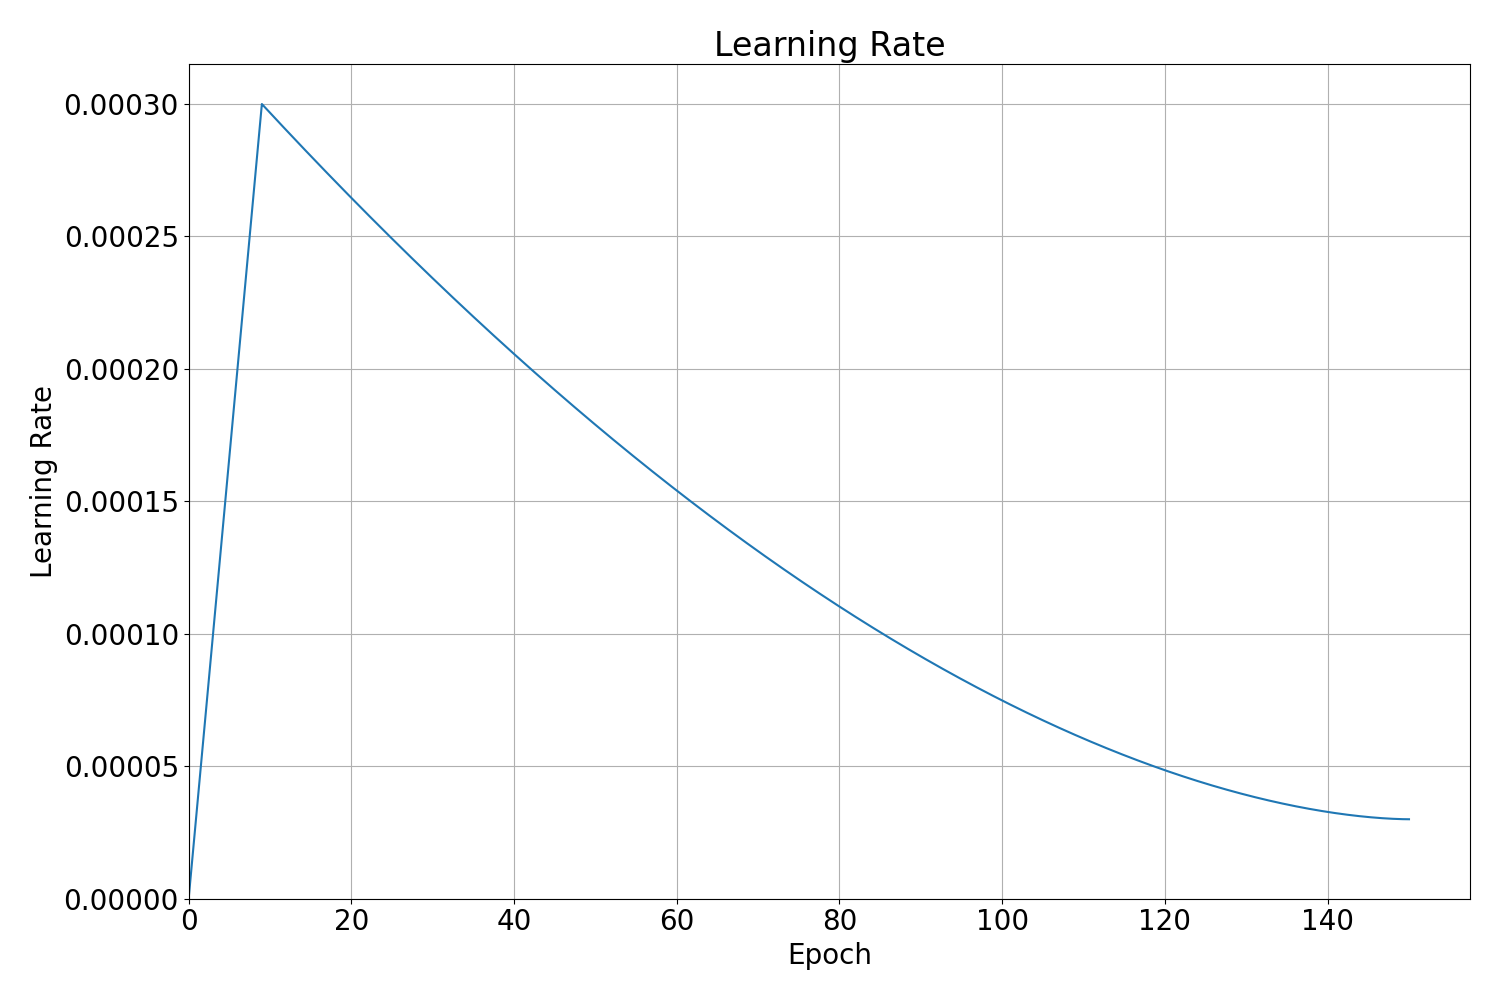
\includegraphics[width=.6\textwidth]{lr}
    \caption{Learning rate during the pretraining.}
    \label{fig:lr}
\end{figure}\noindent

\paragraph{Accuracy measures}
In order to measure the performance of the pretraining model, the accuracy of word and entity predictions are calculated throughout the training.
Due to the size of the classification problem, especially regarding entities, top $ k $ accuracies are calculated - that is, if the true token was among the $ k $ tokens given the highest probability by the model.
Top 1, 3, 5, and 10 accuracies are calculated for both the masked word and masked entity task using every example that the model trains on, while top 25 and 50 are calculated using one twentieth of examples for computational efficiency.

\subsection{Fine-tuning DaLUKE for Named Entity Recognition}%
\label{sub:fine-tune-ner}
The fine-tuning of DaLUKE largely followed that of LUKE, described in section \ref{sec:LUKE}.
The main DaLUKE NER model was produced by fine-tuning on DaNE.

After each epoch, the model was evaluated on the development split of the dataset.
When a better score than the hitherto best checkpoint was found, the checkpoint was overwritten.
The best checkpoint of the model was used for evaluation on the test set.

\paragraph{Learning rate}
Unlike in the pretraining, we did as Yamada et al. and used a slanted triangle learning rate \cite{yamada2020luke}.
Howard and Ruder have also shown that the slanted triangle approach for fine-tuning tasks improve results over a linear decaying learning rates without warmup \cite{howardruder2018universal}.

\paragraph{Loss}
Due to the nature of the $ n $-grams, only very few spans actually cover entities, making the O class dominate the dataset.
For instance, in the training set of DaNE, the O class accounts for 99.3\pro\ of spans.
Furthermore, the actual entities themselves are not perfectly balanced as all things should be.
This motivated us to implement class frequency-weighted, the performance of which is discussed in section \ref{subsec:lossexp}.

The class-weighted loss $ l_w $ was calculated similarly to the unweighted loss in equation \eqref{eq:crossentropyloss}:
\begin{equation}\label{eq:w-crossentropyloss}
    l_w = \frac{1}{\sum_{j=1}^{C} w_j}
    \sum_{i=1}^N w_{c_i} \left(
        -X_{i, c_i} + \log \sum_{j=1}^C \exp X_{i, j}
    \right)
\end{equation}
where $ w_j $ is weight of class $ j $ \cite{pytorchcel}.
We used the reciprocal of the number of occurrences of each class in the training dataset.

Unless otherwise stated, all fine-tunings presented in the rest of the report use the non-weighted loss.

\paragraph{Hyperparameter search}
The development set of DaNE was used to guide a simple search for fine-tuning hyperparameters for the final model.
The search is performed by repeating the training procedure with all combinations of the following parameter values that were chosen based on previous, informal experimentation.
\begin{enumerate}
    \item Batch size $\in\{8, 16\}$
    \item Peak learning rate $\in\{10^{-5}, 5\ctp{-5}\}$
    \item Dropout (final, linear layer) $\in\{0.025, 0.1\}$
    \item Whether or not to use class-weighted loss $\in\{\text{Yes}, \text{No}\}$
\end{enumerate}
For each combination, the resulting model was evaluated on the development set, shown in Table~\ref{tab:hyperres}, and the hyperparameters with highest average F1 score was chosen.
The final model was produced by fine-tuning again to limit selection bias.
The chosen hyperparameters are reported on Table~\ref{tab:main-hyper} together with the used hyperparameters that were not tested.
\begin{table}[H]
    \centering
    \small
    \begin{tabular}{l|r}
        Parameter                       & \jl{Value}\\\hline
        Epochs                          & 15\\
        Batch size                      & 8\\
        Peak learning rate              & $5\ctp{-5}$\\
        LR warmup steps proportion      & $ 6\pro $\\
        Dropout (pretrained model)      & $ 0.1 $\\
        Dropout (final, linear layer)   & $ 0.025 $\\
        Weight decay                    & $ 0.01 $\\
        Loss weighting                  & No
    \end{tabular}
    \caption{Hyperparameters used for fine-tuning DaLUKE for named entity recognition.}
    \label{tab:main-hyper}
\end{table}\noindent

\subsection{Implementation Details and Open Source Software}%
\label{sub:oss}

\paragraph{Open Source Software Package}
We publish DaLUKE and all related code under the MIT open source software license \cite{mitlicense}.
All code and documentation is available at \url{https://github.com/peleiden/daluke}.
The pretrained model is available with MLM layers at \url{https://nx5746.your-storageshare.de/s/qDM2TE6m9CKmPWd}.
The model fine-tuned on DaNE is available at \url{https://nx5746.your-storageshare.de/s/wxbY3TrwfAoYxb9}.
Our software package is \code{pip} installable and runs on Python 3.8 and above.
Simply run \code{pip install daluke} to install it on your computer.
It allows for using DaLUKE both for MLM and NER on text files or inputted strings directly from the command line.
For instructions, see the read-me fill on the repository.

\paragraph{Implementation}
Yamada et al. have made their code\footnote{\url{https://github.com/studio-ousia/luke}. Visited June 11, 2021.} freely available under the Apache License 2.0 \cite{apachelicense}.
We highly appreciate this, and our original plan was to base our implementation on this.
However, we quickly ran into a number of issues with this approach:
Getting all dependencies installed with the correct versions on our computing cluster proved to be a very challenging task.
To solve this, we forked the repository and updated both Python and several of the dependencies to newer versions, but this in itself required significant code rewrites.
When that worked, we started pretraining, which presented more mysterious issues:
Training on a single GPU worked, but two GPU's slowed training by a factor of three, and three or more GPU's simply did not work.
Due to limited GPU availability, cryptic error messages, and an almost complete lack of documentation, debugging once again became difficult.

These reasons compelled us to reimplement the model and training from scratch.
This allowed us to fit the software to our needs and gave better insight into the LUKE method.
The forked LUKE repository, available at \url{https://github.com/peleiden/luke}, is used for parts of the dataset preparation, but everything else has been reimplemented.
Our code is inspired from the original LUKE code, but we have made efforts to make it more approachable by making the code more readable and better structured and especially by increasing the amount of documentation.

Rewriting code bases always carries a risk of introducing bugs.
Despite borrowing heavily from Yamada et al., we did introduce a number of bugs in the code that had to be fixed, forcing multiple restarts of the training.
These ranged from domain specific such as accidentally leaving category pages in the entity vocabulary to classical ones such as copying pointers instead of the memory stored at them.
In that regard, using the original code would be safer, as this has been proven to work.
However, given our results, we feel confident that we managed to iron out all major bugs.

\paragraph{Floating Point Precision}
The model was trained using PyTorch Automatic Mixed Precision (AMP) \cite{pytorchamp}, which -- ideally, at least -- should decrease training time with little to no penalty to accuracy \cite{huang2020amp}.
This is partially due to half-precision calculations being simpler, and partially due to the lower memory requirements, allowing larger subbatches and thus better GPU utilization.
However, as Figure \ref{fig:runtime} shows, AMP works as intended when training on NVIDIA Tesla V100's, but had the opposite effect when training on NVIDIA A100's.

AMP works by automatically casting parts of the model to half precision rather than the usual single precision.
Some layers are more sensitive than others to precision.
For instance, linear layers are always casted to half precision, but the loss is calculated using single precision.
Due to the smaller precision, underflow in the gradients is a risk.
This is handled by scaling up the loss and then scaling down the gradients accordingly.
\cite{pytorchamp}

\paragraph{Distributed Training and Runtime}
As transformer training requires significant compute, distributing the training over multiple GPU's can yield significant speedups.
Especially given the parallelizable nature of the transformer compared to recurrent neural network variations \cite{vaswani2017att}, training should scale fairly well on multiple GPU's.

The pretraining took roughly a week.
Due to varying GPU availability, varying numbers of A100's and V100's were used for pretraining and the experiments in section \ref{sec:pretrainpls}.
The main pretraining took approximately a week and used 2-4 V100's.
For comparison, Yamada et al. trained LUKE using 16 V100's over a period of 30 days. \cite{yamada2020luke}

We measured the time needed to train for one epoch on different cluster configurations.
The results are shown on Figure \ref{fig:runtime}.
\begin{figure}
    \centering
    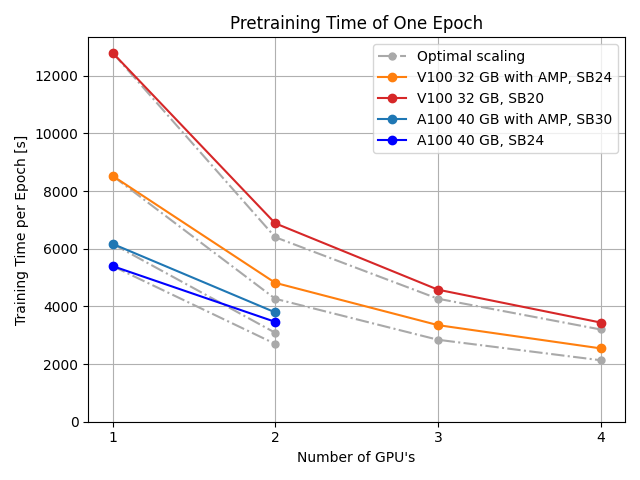
\includegraphics[width=.7\textwidth]{runtime}
    \caption{
        How GPU models, the number of GPU's, and AMP influences pretraining runtime.
        Sub-batch size (SB) is included, as it is important for GPU utilization.
        The measurements were taken with da-BERT weights locked.
        The V100's act mostly as expected with close to optimal scaling and AMP decreasing runtime.
        Surprisingly, however, the A100's, while faster, scale poorly and are slower when using AMP.
        The poor scaling is partially explained by Amdahl's law \cite{klein2011amdahl}: The sequential parts of the code do not get faster along with the GPU and so take up a relatively larger amount of the runtime.
        The A100's also do not have an NVLink bridge unlike the V100's and must therefore communicate over PCIe, which is slower.
        The poor AMP performance, however, is harder to explain.
        According to Hans Henrik Sørensen, DTU Computing Center, it is caused by different \code{gemm} implementations, but we have not investigated it any further.
        Python 3.8.4 using PyTorch 1.8.1 compiled with CUDA 11.1 was used.
    }
    \label{fig:runtime}
\end{figure}\noindent


\end{document}
